\chapter{绪论}\label{chap:introduction}

\section{研究背景}\label{sec:ResearchBackground}

随着机器视觉、计算机图形学、人工智能等众多技术领域的发展,人们对与真实世界多样化交互的需求不断增加,增强现实(Augmented Reality,简称 AR)
能够将图文资料、音频视频、模型动画等虚拟信息通过虚实融合技术叠加显示到真实场景恰当位置处,以此提升用户与真实环境之间的交互体验。
近些年,增强现实广泛应用于科普教育、军事仿真、文化旅游、医养健康、装备维保等众多领域,许多世界顶级的研究机构纷纷开展增强现实
相关技术的研究,发布了 Microsoft HoloLens、Meta 增强现实头盔、Google ARCore/Tango、Apple ARKit等一系列激动人心的AR相关
产品及平台,增强现实技术正处于高速发展之中。
\begin{figure}[!htbp]
    \centering
    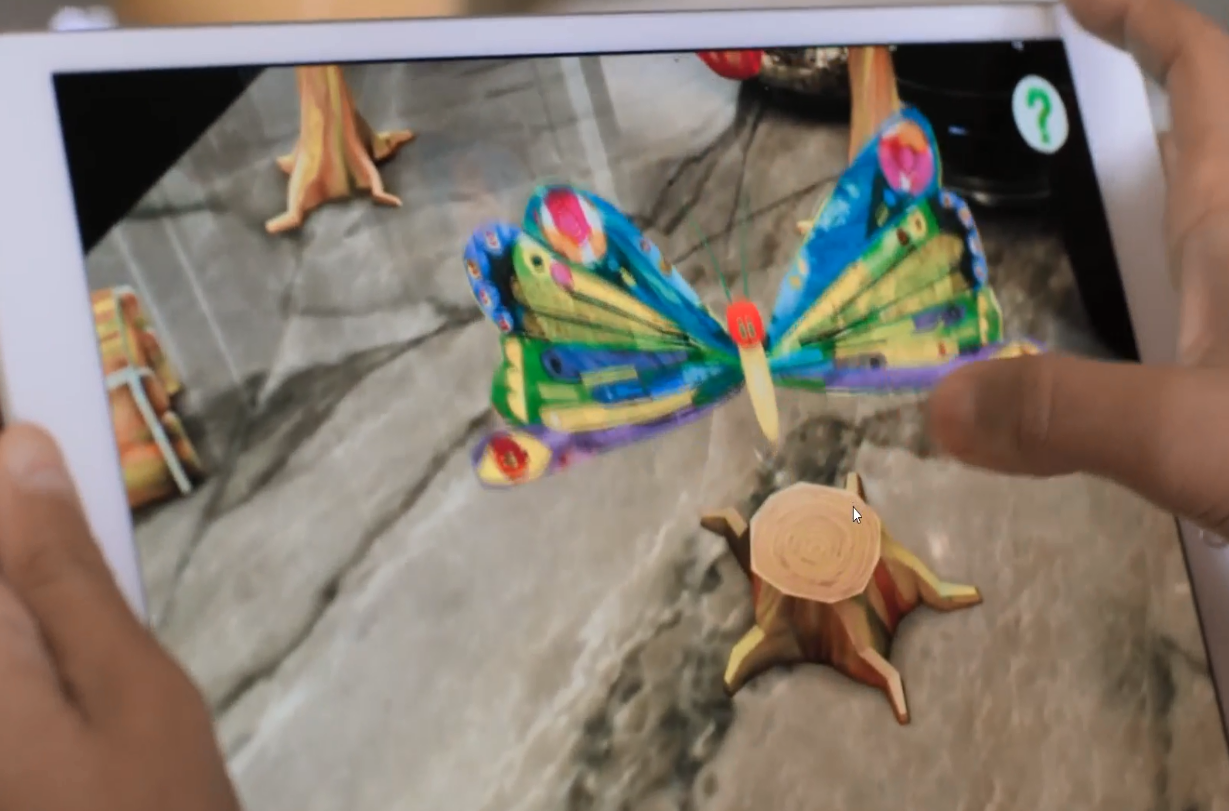
\includegraphics[width=\textwidth]{Img/1-ARExample.png}
    \bicaption{AR用于儿童教育行业。}{AR application for children education.}
    \label{fig:ARExample}
\end{figure}

\begin{figure}[!htbp]
    \centering
    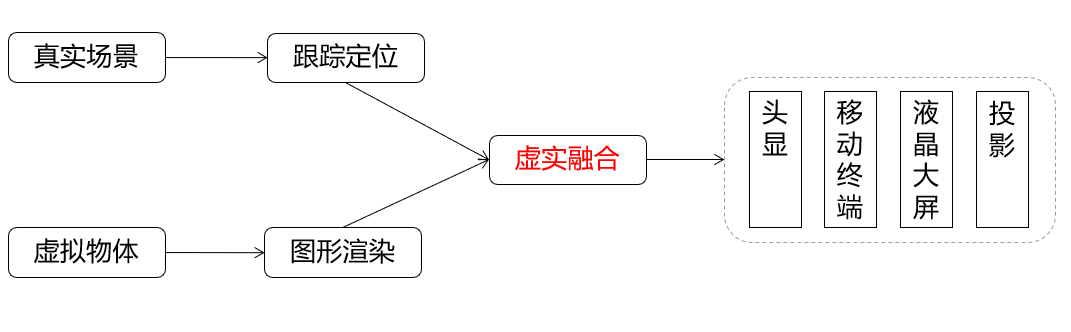
\includegraphics[width=\textwidth]{Img/1-ARflow.png}
    \bicaption{AR系统工作流程图。}{Work flow of AR system.}
    \label{fig:ARflow}
\end{figure}

增强现实系统的工作流程如图~\ref{fig:ARflow}所示。系统根据机器视觉技术在对相机跟踪定位,得到相机在真实场景中的位姿,通过虚实融合技术,
把通过计算机图形学技术渲染得到虚拟信息注册到真实场景中的恰当位置,将虚拟信息与真实场景相结合的结果呈现在头显、液晶屏等终端上,
提供虚实结合的交互效果。

能否精准地通过跟踪注册,将虚拟物体放置在真实场景中,很大程度上影响了增强现实系统能否给予虚拟图形准确的空间定位、物理遮挡、
透视形变、光照阴影等效果,进而决定着系统呈现的真实感和交互体验,这其中关键技术便是虚实融合技术。虚实融合技术是感知环境信息,
将渲染生成的虚拟信息与现实场景精准匹配、叠加的技术。具体来说,虚实融合技术可以从以下几个方面影响增强现实系统的真实感:

{
\setlist[enumerate]{}% restore default behavior
\begin{enumerate}[nosep]
    \item 时间一致性\\基于时间一致性的虚实融合主要关注增强现实系统的实时交互能力,确保虚拟物体与真实物体的运动关系相互协调,
    在时间序列上消除偏差,使得增强现实应用流畅、平滑、无延迟。
    \item 几何一致性\\基于几何一致性的虚实融合主要关注遮挡问题与物理约束,将虚拟信息在真实场景中精准定位。解决虚实遮挡问题
    依赖于对场景三维结构的了解,需要判断真实场景中的物体距离相机的距离,以及被遮挡部分的空间结构信息。物理约束方面,
    主要是约束虚拟物体与真实场景物体不重叠,保证虚拟物体的刚体结构及物理形变。
    \item 光照一致性\\基于光照一致性的虚实融合是根据虚实位置关系,渲染真实性强的光影关系,给虚拟物体添加与真实环境相适应的明暗、阴影等光照效果。
\end{enumerate}
}

我的研究主要集中于几何一致性的虚实融合方面,其关键是相机的跟踪注册技术。跟踪注册技术分为两方面,跟踪即估计相机在场景中的位姿,
得到每个时刻相机于三维场景中的相对位置和朝向。注册即获取场景的三维结构信息,同时将虚拟图形准确注册至真实环境,根据维场景空间
结构信息,准确在目标位置叠加虚拟图像。
\begin{figure}[!htbp]
    \centering
    \begin{subfigure}[b]{0.45\textwidth}
      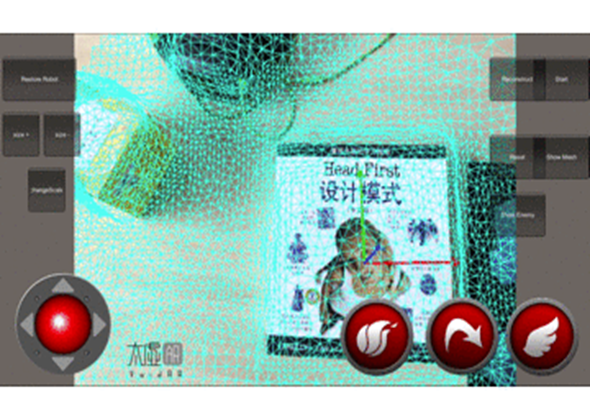
\includegraphics[width=\textwidth]{Img/1-senceUnderstand.jpg}
      \caption{}
      \label{fig:senceUnderstand}
    \end{subfigure}%
    ~% add desired spacing
    \begin{subfigure}[b]{0.45\textwidth}
      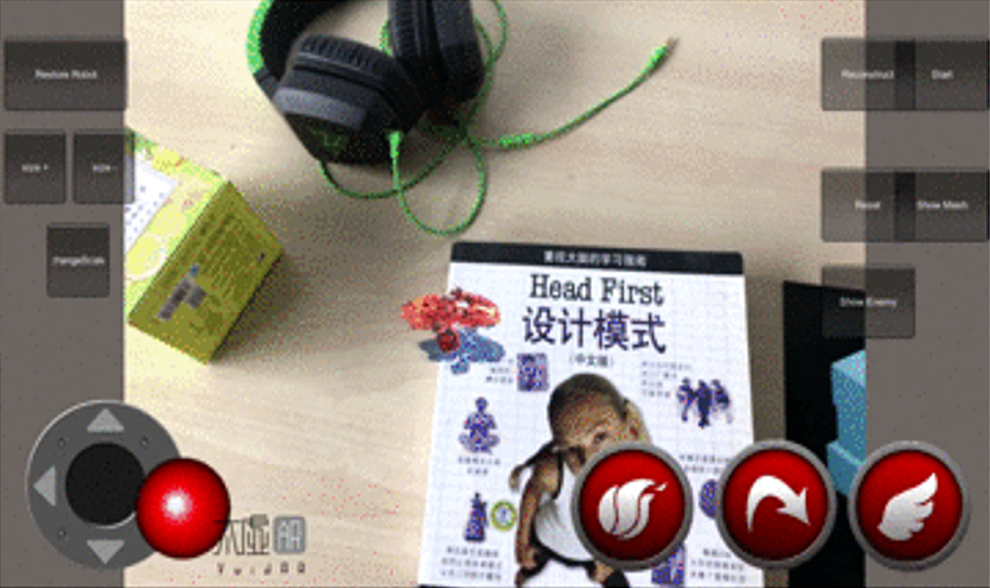
\includegraphics[width=\textwidth]{Img/1-senceUnderstandAR.png}
      \caption{}
      \label{fig:senceUnderstandAR}
    \end{subfigure}
    \bicaption{基于场景理解的AR系统。(a) 场景理解,(b) 虚拟物体跟踪注册。}{AR system based on scene understanding. (a) Scene understanding, (b) Virtual object registration.}
    \label{fig:scene}
\end{figure}

近年来,随着SLAM技术的高速发展,基于场景理解的跟踪注册技术逐渐成为一种新兴解决方案,图\ref{fig:scene}展示了一个基于场景理解的增强现实系统。SLAM(Simultaneous localization and mapping)技术全称即时定位与地图
构建,其目标是在未知环境下,通过相机、激光、惯性单元等传感器不断捕捉环境信息,实时的同步进行相机自身位姿的估计和未知环境的
三维地图构建。其中,以摄像机为数据获取源,基于特征匹配的视觉SLAM(Visual SLAM,V-SLAM)因其硬件需求较低,便携性更高,
在增强现实领域拥有更多应用空间。通过视觉SLAM技术,能够在未知场景下,无需提前布置或录入标志信息,同步获取高精度的跟踪定位结果和
三维环境感知结果,从而提供增强现实系统对于环境在三维层面的理解能力,从而提高跟踪注册精度。

然而,基于特征匹配的传统视觉SLAM技术仍存在一些问题:
{
\setlist[enumerate]{}% restore default behavior
\begin{enumerate}[nosep]
    \item 语义信息利用不充分\\传统SLAM系统并没有完全利用图像所蕴含信息,如高层的语义分割,物体级的目标检测等信息,仅提取了二维图像的局部特征。
    在位姿估计过程中,局部特征匹配提供的约束不够充分,所建地图仅能描述三维空间的几何结构,没有提供语义层面的表达。
    \item 难以应对动态场景\\在动态环境下,因基于视觉匹配的算法和硬件的限制,大多数传统视觉SLAM系统难以处理剧烈变化的动态环境,例如移动的人或物体,很容易
    大幅度影响相机位姿估计的表现,甚至诱发系统崩溃。同时在建图方面,传统视觉SLAM系统大多面向静态环境增量式建图,对于运动的物体
    易出现目标重影、模糊等问题。
\end{enumerate}
}

随着深度学习技术的发展,高层语义信息可以方便地通过卷积神经网络(Convolutional Neural Network,CNN)得到。通过
卷积神经网络,可以基于海量数据训练模型,完成目标检测、语义分割等任务,检测目标图像中的物体,输出其类别与位置,将每个
二维像素点赋予类别标签,给予其可解释的类别。

近年来,一些相关工作将深度网络与视觉SLAM框架相结合,能够识别环境中的独立个体,在传统视觉SLAM框架所建立的三维地图的基础上,
关联语义信息与几何信息,以此丰富三维地图的信息表达,建立具有语义信息和空间结构信息的场景地图,提高感知等级。同时能够在相机位姿估计过程中,根据语义信息提供更丰富的约束,
得到更精准的相机跟踪定位结果,并增强系统在动态环境下的鲁棒性。此类方法可称作语义SLAM(Semantic SLAM),它不但能够帮助系统
解决“目标在哪”的问题,还能够进一步明确“目标是什么”,是当前研究的热点和难点。

因此,语义SLAM技术能够帮助传统视觉SLAM框架提升位姿估计精度、动态场景下的鲁棒性和地图信息表达能力,进而能够帮助增强现实
系统在静态或动态场景下准确理解环境,计算得出虚拟信息在场景中应叠加投放的准确位置,提升跟踪注册的精度,用于优化增强现实系统中的虚实融合问题,
提高增强现实应用的真实感。因此,以上所述的传统视觉SLAM系统存在的问题,也是增强现实系统中基于场景理解的跟踪注册技术所面临的难点问题。
对于语义SLAM进行的研究,在增强现实领域具有一定的现实意义和应用价值。    

\section{国内外研究现状}\label{sec:ResearchStatus}
近年来,随着视觉SLAM系统的不断发展完善,其对于语义信息的利用也经历了从低层至高层的发展。以最初的低层局部特征为基础,发展出了
结构化的特恒工程,而后又开展了结合高层语义信息的语义映射和动态环境下的SLAM的研究。在增强现实领域中,语义SLAM相关研究更注重于
对环境的高层理解与表示,以及在动态环境下系统鲁棒性的和相机位姿估计精度的提升。
\subsection{传统SLAM框架}
传统SLAM框架大多包含负责跟踪的前端和负责优化的后端两大主要模块,其中前端模块按照特征提取方法可分为特征点法和直接法两类,后端模块
又可根据优化方法分为基于滤波的方法和基于非线性优化的方法两类。早期SLAM框架大多包含基于特征点法的前端模块和基于滤波方法的后端模块。
Andrew J Davison等人于2007年提出的MonoSLAM是基于特征点的SLAM的先驱之作,它通过扩展卡尔曼滤波
(Extended Kalman Filter,EKF)进行后端优化,保证了单目SLAM的实时性,但只能应用于较小的场景。随后,Klein 与 Murray 等人开创性地采用基于非
线性优化的方法以克服滤波技术的局限,提出了PTAM\citep{Klein2007Parallel}系统,将跟踪与建图作为两个分开的线程,获得更加稠密与更大范围的场景结构,
无论在精度还是鲁棒性等方面都取得了比基于滤波的方法更好的表现,但在处理的场景规模和稳定性方面仍有提升空间。

PTAM的思想奠定了SLAM领域研究的方向和基础,在此之后,众多研究机构提出了很多当前性能优秀的SLAM框架。西班牙Zaragoza大学的Raúl Mur-Arta
等人于2015年提出的ORB-SLAM\citep{mur2015orb}首次将地图初始化、视觉里程计、后端优化、闭环检测等模块集成至一个完整系统,其主要思想是
对相机捕获的图像提取ORB\citep{Rublee2012ORB}特征并在连续帧间进行特征匹配,构造重投影误差并以非线性优化的方法进行优化。
而后其在2017年又提出了ORB-SLAM2\citep{mur2017orb},更进一步加入了重定位模块,成为现今最为完整、高效的基于特征点的稀疏SLAM系统之一。
与之不同,Jakob Engel等人在2014年提出了基于直接法的LSD-SLAM\citep{Engel2014LSD},此方法无需图像特征提取与匹配,而是基于像素间的光度误差直接优化,
并进行半稠密的重建。随着RGB-D相机的发展,基于深度数据的SLAM系统亦开始涌现。帝国理工大学的Thomas Whelan等人在2015年提出了
ElasticFusion\citep{whelan2015elasticfusion},此方法采用几何误差和光度误差联合优化,使用面元结构建模,在不断优化迭代中
提高位姿估计和地图构建精度。

然而,这些方法都仅通过低层的局部特征匹配或像素匹配来构造约束、进行优化,所建地图也仅限于几何层面,没有结合高层语义信息。此外,
这些方法都面向静态环境,在动态场景下,其相机位姿的估计精度将受到很大影响。

\subsection{语义映射}
传统SLAM构造的三维地图仅包含几何信息,难以满足复杂的任务需求。语义映射能够将二维语义信息与三维几何地图相关联,逐渐成为了一个
热门的研究领域。这类工作通过深度网络或几何方法对二维图像帧进行语义分割,获取像素级的语义标签,再通过特定规则与三维路标点关联匹配,
以构造同时含有语义信息和几何信息的三维地图。

同样来着帝国理工大学的工作SemanticFusion\citep{MccormacSemanticFusion}以它使用ElasticFusion为基础,使用FCN\citep{long2015fully}进行
语义分割,同时使用条件随机场(Conditional Random Field,CRF)优化分割结果,语义匹配方面,使用贝叶斯更新方法将二维语义与三维地图进行数据关联,
系统除构建了语义地图外,还验证了SLAM系统所捕获的连续帧能够辅助优化二维语义分割结果。
来自东南大学的Li X等人\citep{LiSemi}使用深度网络模型DeepLab-v2\citep{Chen2014Semantic}进行二维图像的语义分割,该网络结构包含
孔洞卷积和空间池化金字塔(ASPP),辅以条件随机场进行地图正则化,能够平滑语义分割结果中的噪声。此方法同样使用贝叶斯更新方法
进行数据关联,结合LSD-SLAM,解决了室内、室外不同场景下的尺度问题,其构建的语义地图也有一定精度提升。来自国防科技大学的Qi等人\citep{qi2018deep}
使用点云建图,并关联语义标签,并通过图分割方法将点云分为聚类的超体,迭代获取更精细的平面部分,优化了语义建图的细节。
除此之外,Hoang等人\citep{hoang2019high},Zeng等人\citep{zeng2018semantic}以及CNN-SLAM\citep{tateno2017cnn}等工作都从不同
角度提升了语义关联或语义建图的精度。

这些方法使用的语义信息为像素级别,对于优化相机位姿估计或辅助增强现实应用开发的提升价值有限。在此之上,实例级的语义分割信息
同时包含物体级的目标检测结果和像素级的语义分割结果,有着更高的研究价值和应用潜力。N. Sunderhauf等人\citep{S2017Meaningful}
使用物体识别框架SSD\citep{Liu2016SSD}进行目标检测,对关键帧图像生成固定数量的物体框,并给出目标分类结果和置信度。
语义分割部分则选择了使用基于超体元的分割点云模型,通过最近邻方法将目标检测结果映射到分割后的点云模型上,得到具有物体级标签的语义地图。
Fusion++\citep{mccormac2018fusion++}使用稠密SLAM系统KinectFusion\citep{Newcombe2011KinectFusion}中的三维重建方法,
结合同步进行目标检测、语义分割的深度网络Mask R-CNN\citep{HeMask},将二维图像检测到的物体以TSDF(Truncated Signed Distance Function)
方法增量式建立三维模型,得到物体级的语义地图。

然而以上方法仅单纯地将二维语义信息与三维几何地图进行了关联映射,并未利用语义信息优化SLAM的核心任务之一——状态估计。此外,
这些工作仅面向静态环境开展,传统视觉SLAM在动态环境下面临的位姿估计不准、建图出现重影等问题,在这些系统中依旧存在。

\subsection{动态环境下的SLAM}
SLAM系统所面对的困难场景之一是动态环境,三维物体的运动和相机自身的抖动都可能为状态估计环节引入误差,也会使得所建的三维地图出现重影等问题。
现有的一些传统视觉SLAM算法在这方面还很比较薄弱,而一些近期的工作开始尝试利用语义信息来解决这些问题。

2018年帝国理工大学提出的MaskFusion\citep{runz2018maskfusion}也使用Mask R-CNN进行实例分割,同时针对网络分割结果的边缘不精确
问题,使用了几何方法在二维图像上进行细化边缘,与深度网络的分割结果相结合,得到物体级的语义标签。此方法能够对前景物体单独建模、
跟踪和维护,实现了动态场景下的物体级建图,但MaskFusion并未解决动态环境对位姿估计带来的误差问题。
来自清华大学的Yu等人提出了DS-SLAM\citep{YuDS},利用SegNet\citep{VijaySegNet}实时获取像素级的语义标签,结合基于光流的运动一致性
检测方法来滤除场景中如行走的人等的动态部分的特征点,依次减少动态目标对于位姿估计的影响。然而此方法仅使用了像素级的语义分割结果,
没有进行物体级建图,此外,仅滤除了属于“人”这一个类别的动态目标的特征点,没有考虑不同类别物体的影响。
Berta等人于2018年发表的DynaSLAM\citep{BertaDynaSLAM}能够通过多视图几何、深度学习或二者结合的方法检测场景中的运动物体,
并将属于运动目标范围内的特征点移除,从而提高位姿估计精度。但这种方法粗暴地移除了属于某一语义类别的全部特征点,容易因剩余特征点
数量过少而导致跟踪失败,而与DS-SLAM相似,DynaSLAM没有考虑不同类别物体的影响,也没有建立动态环境下的物体级语义地图。

这些方法都为克服传统视觉SLAM在动态场景下的局限,结合语义信息做出了一些努力,取得了相应成果。但它们没有完全利用语义信息,
同时优化位姿估计和建立物体级语义地图,在这一方面仍有很大的研究空间,需要后续的大量实验和探索。

\section{论文主要研究内容}
基于目前所积累的理论知识、研究思路和实验数据,本文对基于语义SLAM,对动态场景下位姿估计优化方法、语义地图的构建和表示方法及
在增强现实系统中的应用方法进行了研究,力图以基于语义信息的SLAM改进方法为核心技术,提高增强现实系统的虚实融合性能,
提升系统的真实感体验,解决一系列涉及到的问题。
\begin{figure}[!htbp]
    \centering
    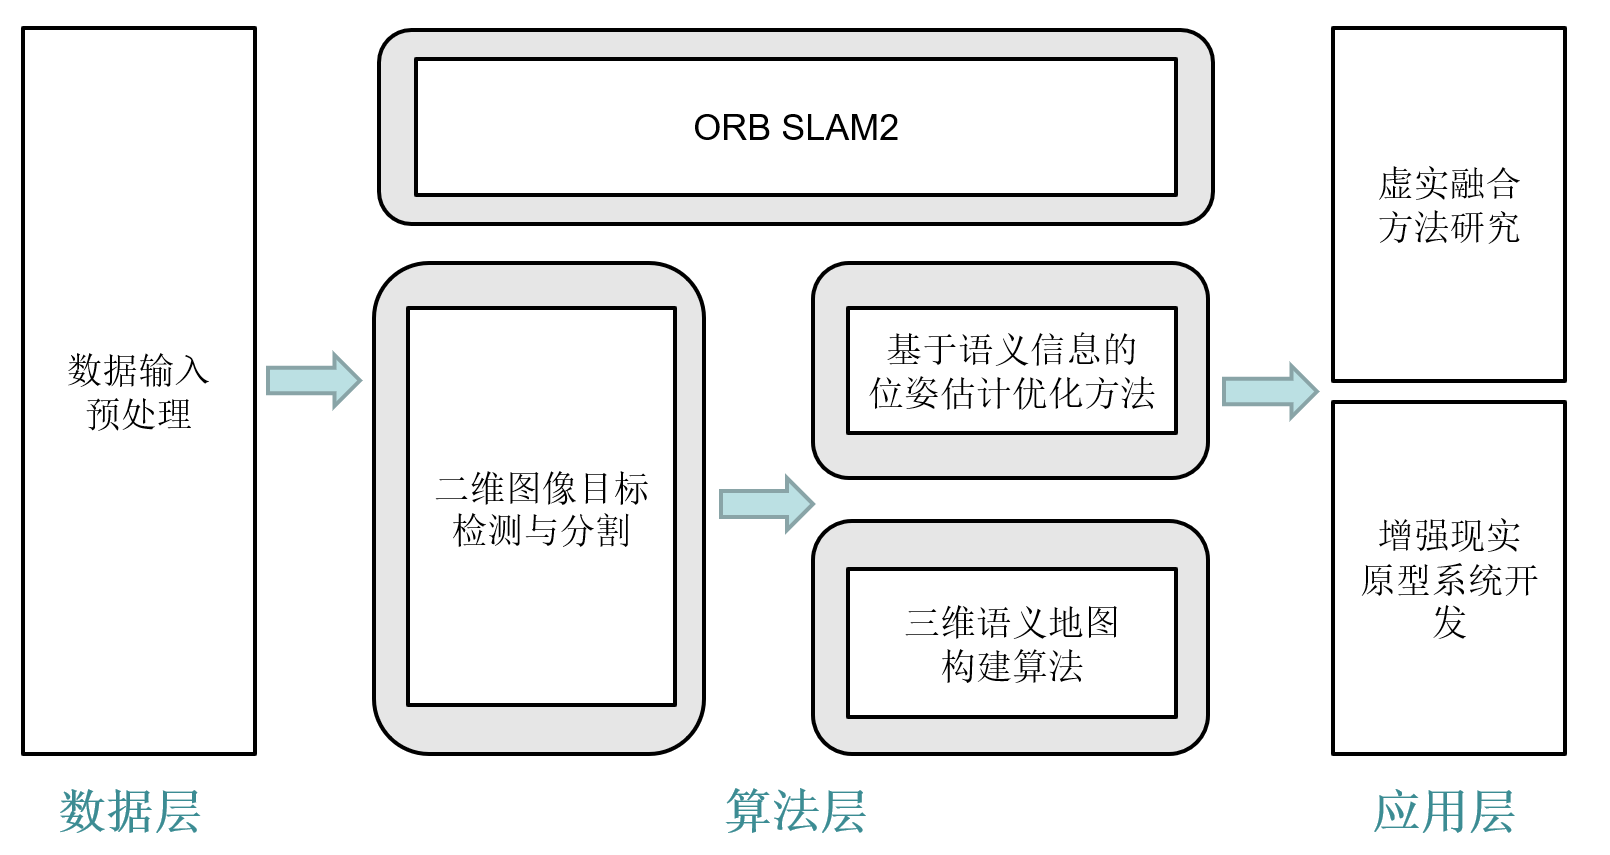
\includegraphics[width=\textwidth]{Img/1-researchFramework.png}
    \bicaption{系统研究框架。}{Research framework of this paper.}
    \label{fig:researchFramework}
\end{figure}
本文工作主要体现在以下几个方面:
{
\setlist[enumerate]{}% restore default behavior
\begin{enumerate}[nosep]
    \item 动态场景下基于语义信息的位姿估计优化方法\\这部分研究工作针对动态场景,提出了双阶段的动态外点滤除算法,此算法结合基于语义类别的
    自适应权重生成方法和基于极线约束的动态一致性检测方法,能够对于不同类别的物体自适应生成不同的判定条件,判断其是否处于运动状态,
    并移除处于运动状态的物体的轮廓内的特征点。此算法在TUM RGB-D数据集上进行了验证,在动态场景下其结果比ORB-SLAM2有数量级式的提升,
    提升幅度在大部分指标上优于业界先进系统,表明它能够有效减少环境中运动物体对于SLAM系统位姿估计的干扰,提升基于特征的视觉SLAM系统在动态场景下的位姿估计精度和鲁棒性。
    \item 语义地图的构建和表示方法\\这部分研究工作针对不同层级语义地图对环境的表示能力,分别探究了基于局部特征的预置语义库地图和语义SLAM系统生成的
    物体级三维语义点云地图的构建和表示方法。对于预置语义库地图提出了特征识别和跟踪方法,验证了其对室外环境的表示能力和在增强现实导航系统中的应用能力。
    对于物体级三维语义点云地图,本文提出了针对语义类别的物体跟踪策略,能够对环境中的物体分别建模、跟踪,适应动态变化的环境,并进行语义关联。
    此方法在动态环境和静态环境下分别进行了验证,结果表明它能够提高建图的鲁棒性,建立随环境变化而变化的物体级语义地图,从而提高对三维环境的表示能力。
    \item 增强现实原型系统的设计与实现\\这部分研究工作设计并实现了一个增强现实原型系统,融合了述研究的算法,在虚实融合阶段进行了
    优化,提升了系统的真实感体验。
\end{enumerate}
}

\section{论文组织结构}
第一章介绍了本文研究的背景和意义,详细列举了国内外相关研究现状,明确了本文的研究工作并给出了本文的章节安排。

第二章从整体上介绍了本文所提出系统的框架结构,包括所用的视觉SLAM框架、深度神经网络以及本文所设计的结合二者的语义SLAM框架。

第三章详细描述了本文所研究的动态场景下基于语义信息的位姿估计优化方法,给出了此算法在公开数据集的测试数据,与当前主流视觉SLAM框架和
先进同类方法进行了对比分析。

第四章聚焦语义地图的构建和表示方法,分别叙述了基于局部特征的预置语义库地图和物体级三维语义点云地图的构建和表示,并
对其效果分别进行了评估。

第五章介绍了本文基于算法理论研究,设计并实现的增强现实原型系统,给出了其在虚实融合方面的性能和真实感体验的测试与分析。

第六章对于本文所述的全部工作进行了整体总结,分析了当前存在的不足和提升空间,列出了后续应开展的工作内容,对未来研究前景进行了展望。
